\documentclass[11.5pt]{sig-alternate} % sets document style to sig-alternate
% packages
% typesetting
%\usepackage{dirtytalk} % typset quotations easier (\say{stuff})
\usepackage{hanging} % hanging paragraphs
\usepackage[defaultlines=3,all]{nowidow} % avoid widows
\usepackage[pdfpagelabels=false]{hyperref} % produce hypertext links, includes backref and nameref
\usepackage{xurl} % defines url linebreaks, loads url package
\usepackage{microtype}
\usepackage{textgreek}
%\usepackage{textcomp}
%\newcommand{\texttildemid}{\raisebox{0.4ex}{\texttildelow}}
% layout
\usepackage{enumitem} % control layout of itemize, enumerate, description
\usepackage{fancyhdr} % control page headers and footers
\usepackage{float} % improved interface for floating objects
%\usepackage{multicol} % intermix single and multiple column pages
% language
\usepackage[utf8]{inputenc} % accept different input encodings
\usepackage[english]{babel} % multilanguage support
% misc
\usepackage{graphicx} % builds upon graphics package, \includegraphics
%\usepackage{lastpage} % reference number of pages
%\usepackage{comment} % exclude portions of text (?)
\usepackage{xcolor} % color extensions
\usepackage[backend=biber, style=apa]{biblatex} % sophisticated bibliographies % necessary for HTML to display author info and date on abstract page
\usepackage{csquotes} % advanced quotations, makes biblatex happy
\usepackage{authblk} % support for footnote style author/affiliation
% tables and figures
\usepackage{tabularray}
\UseTblrLibrary{varwidth}
%\usepackage{array} % extend array and tabular environments
\usepackage{caption} % customize captions in figures and tables (rotating captions, sideways captions, etc)
%\usepackage{cuted} % allow mixing of \onecolumn and \twocolumn on same page
\usepackage{multirow} % create tabular cells spanning multiple rows
%\usepackage{subfigure} % deprecated, support for manipulation of small figures
%\usepackage{tabularx} % extension of tabular with column designator "x", creates paragraph-like column whose width automatically expands
%\usepackage{wrapfig} % allows figures or tables to have text wrapped around them
%\usepackage{booktabs} % better rules
% dummy text
%\usepackage{blindtext} % blind text dummy text
%\usepackage{kantlipsum} % Kant style dummy text
\usepackage{lipsum} %lorem ipsum dummy text
% other helpful packages may be booktabs, longtable, longtabu, microtype

\pagestyle{fancy} % sets pagestyle to fancy for fancy headers and footers

% header and footer
% modern way to set header image
\renewcommand{\headrulewidth}{0pt} % defines thickness of line under header
\renewcommand{\footrulewidth}{0pt} % defines thickness of line above header
\setlength\headheight{80.0pt} % sets height between top margin and header image, effectively moves page contents down
\addtolength{\textheight}{-80.0pt} % seems to affect the lower height. maybe only works properly if footer numbers enabled?
\fancyhf{}
\fancyhead[CE, CO]{
\includegraphics[width=\textwidth]{headerImage.png}}
% footer
%\fancyfoot[LE,LO]{Article Title Here \\ DOI: }% left footer article title and doi
%\fancyfoot[CE,CO]{{}} % center footer empty
%\fancyfoot[RE,RO]{\thepage} % right footer page numbers
%\pagenumbering{arabic} % arabic (1, 2, 3) numbering in footer

\hypersetup{colorlinks=true,urlcolor=blue} % sets link color to blue
\urlstyle{same} % sets url typeface to same as rest of text

% set caption and figure to italics, label bold, left align captions, does not transfer to HTML
\captionsetup{labelfont=bf, font={large, it}, justification=raggedright, singlelinecheck=false}
\renewcommand\theContinuedFloat{\alph{ContinuedFloat}}

%this next bit is confusing, but essentially changes the width of the abstract. Seems to have been copied from this https://tex.stackexchange.com/questions/151583/how-to-adjust-the-width-of-abstract
\let\oldabstract\abstract
\let\oldendabstract\endabstract
\makeatletter %changes @ catcode to enable modification (in parsep)
\renewenvironment{abstract} %alters the abstract environment
{\renewenvironment{quotation}%
               {\list{}{\addtolength{\leftmargin}{1em} % change this value to add or remove length to the the default ?
                        \listparindent 1.5em%
                        \itemindent    \listparindent%
                        \rightmargin   \leftmargin%
                        \parsep        \z@ \@plus\p@}%
                \item\relax}%
               {\endlist}%
\oldabstract}
{\oldendabstract}
\makeatother %changes @ catcode to disable modification

% checks
% italics
% links
% dashes
% tildes
\begin{document}

\title{An Artificial Intelligence Tool for Accessible Science Education}

\author[1]{\large \color{blue}Jacob Watters}
\author[1]{\large \color{blue}April Hill}
\author[2]{\large \color{blue}Mellissa Weinrich}
\author[3]{\large \color{blue}Cary Supalo}
\author[1]{\large \color{blue}Feng Jiang*}

\affil[1]{Metropolitan State University of Denver}
\affil[2]{University of Nothern Colorado}
\affil[3]{Independence Science}
\toappear{}
%% ABSTRACT
\maketitle
\begin{@twocolumnfalse} 
\begin{abstract}
\item 
\begin{large}
\textit{One of the most important issues in accessible science education is creating a laboratory workspace accessible to blind students or students with visual impairments (VI). Although these students are often provided access to the science lectures, they are usually denied full participation in hands-on laboratory work. Current solutions to this problem focus on providing special accommodations such as asking sighted lab partners to complete the hands-on work. Although the accessibility of laboratory devices in modern science education has been improved in recent years, students with VI often remain passive learners. In this work, we developed a new artificial intelligence tool, the MSU Denver Virtual Lab Assistant (VLA), using Amazon Web Services (AWS), Amazon Alexa Skills Kit (ASK), Alexa smart speaker, and a microcontroller (Raspberry Pi). The VLA can be used as a virtual assistant in the lab in combination with other access technologies and devices. The VLA allows students with VI to perform the hands-on laboratory work by themselves simply using voice control. The VLA can be accessed through any smartphone or Amazon Echo device to assist general science lab procedures. The VLA is designed to be applicable to different science laboratory work. It is also compatible with other common accessible electronic devices such as the Talking LabQuest (TLQ). We believe that the VLA can promote the inclusion of learners with VI and be beneficial to general accessible science education work.}

\item Keywords: Artificial Intelligence, Virtual Assistant, Accessible Science Education.
\end{large}
\end{abstract}
\end{@twocolumnfalse}

\textbf{*Corresponding Author, Feng Jiang}\\
\href{mailto: fjiang@msudenver.edu }{(fjiang@msudenver.edu)} \\
\textit{Submitted  February 1, 2021}\\
\textit{Accepted March 28, 2021} \\
\textit{Published online September 17,2021} \\
\textit{DOI:10.14448/jsesd.13.0010} \\
\pagebreak
\clearpage
\begin{large}
\section*{BACKGROUND}

According to the statistics provided by the U.S. Bureau of Labor Statistics (2020), people with a disability are less likely to work as Science, Technology, Engineering, and Mathematics (STEM) professionals than those with no disability (19.9 percent, compared with 24.9 percent). This suggests that students with disabilities are disproportionately discouraged from pursuing STEM education and employment. For youth with visual impairments (VI), artificial barriers encountered in public school science laboratories (e.g., insufficient hands-on materials, few teachers who understand tactile learning, lack of access to resources) may hinder their entry into the STEM workforce (Supalo, 2005). This lack of access to experiences with direct, hands-on laboratory work leads to the marginalization of students with disabilities in science. In the case of students with VI, the lack of vision requires this population to have spatial awareness and be familiar with the layout of the laboratory workspace. Often, students with VI lack the ability to read essential information (e.g., procedural details, safety data, etc.) required to effectively participate in the STEM laboratory (Field et al., 2003). A common solution to this problem is to pair the student with VI with a sighted lab partner, who is called a “directed assistant” (Miner et al., 2001). This assistant is expected to carry out all tasks requested by the student with VI with the exception of any task that would violate safety protocols. This system puts the student with VI in the role of an expert while the assistant is a subordinate. However, students with VI who are early in their science education may not feel qualified and/or experienced to serve in the role of expert. More importantly, the directed assistant approach creates a passive laboratory experience for the student with VI, who is excluded from participating in the hands-on, active aspect of science laboratory learning. The shift from the directed assistant approach to an independent approach in a hands-on way to promote interest in STEM careers is needed in science education for students with VI (Supalo, 2012).

Access technology (AT) solutions are widely used to help involve students with VI in science learning (Rose et al., 2005). The modern science learning environment is becoming more equipped with accessible and inclusive technologies, such as digital textbooks or learning materials, online course management systems, smartphones, and tablet computers equipped with text-to-speech and voice dictation tools. These tools help students with VI greatly while still not solving some fundamental problems faced in the laboratory workspace. Most AT solutions are effective at transmitting text-based information or generating the voice explanation of collected data. However, they are unable to convey general lab settings, interactively answer questions, give general guidance of lab procedures, perform calculations, or pause after dictating a task until the student is ready to move to the next step. In a laboratory environment, it is common for students with VI to have more anxiety and fear due to the complexity of the lab procedures and the unknown status of all lab materials and devices. Human assistants can reduce stress and fear in such an environment but often take over the operating role of students with VI. Hence, a “smart assistant” with the ability to provide all procedural information step by step, answer general questions, perform calculations, assist in acquiring and recording experimental data, and monitor the status of a measurement device is needed. 

Unlike the aforementioned approaches, an artificial intelligence (AI)-based “smart assistant” can improve the accessibility of the laboratory environment while maintaining the operating role of students with VI. AI is proving itself to be a robust, innovative 21st-century technology that has boundless applications in today's world. In the arena of science education, the use of AI in the science laboratory is in its infancy. The greatest difference between traditional AT tools and AI tools is whether the software or devices are equipped with self-learning abilities. Tools with self-learning abilities can provide a more interactive learning experience and continually improve themselves based on user interactions. We developed the MSU Denver Virtual Laboratory Assistant (VLA) using multiple Amazon Web Services (AWS), an Alexa smart speaker, and a microcontroller (Raspberry Pi) connected to other lab devices. The VLA is equipped with all public Amazon Alexa skills and one new self-developed Alexa skill designed for general science laboratory work. All Amazon Alexa skills can constantly improve themselves while being used by numerous Amazon customers every day. The self-developed skill enables VLA to read and interpret the traditional laboratory document, thus generating interactive voice responses to assist the laboratory work. 

In this paper, we introduce the related tools, hardware, and AWS services used in our work and explain how they were utilized to build the VLA. We also describe the unique features we have designed for our VLA, which make it adaptable to different lab procedures and compatible with other electronic devices. Finally, conclusions and future work directions are given. 

\section*{DESIGN OF THE VIRTUAL LAB ASSISTANT}

\subsection*{Overview of Virtual Lab Assistant}

The VLA system consists of four main components working together to create a single cohesive tool that greatly improves the accessibility of the laboratory environment. These components include an Alexa smart speaker, a custom Alexa Skill that acts as a virtual AI lab assistant, a Talking LabQuest (TLQ) which allows for accessible data collection and statistical analysis (“Talking labquest”, n.d.), and a Raspberry Pi which allows the Alexa Skill to interact with the TLQ, effectively connecting all the components together. The Alexa skill contains all of the software making up the VLA. This skill code is hosted in an AWS Lambda rather than a server, thus allowing the software to be easily maintained with no server upkeep. The skill has several intents that allow students to perform various lab tasks with the assistance of the VLA tool. Students use an Alexa smart speaker (or any smart device such as a smartphone) to provide verbal input to the VLA skill. The input is passed through the Utterance Profiler, which allows the VLA to infer which intent to trigger based on example phrases defined in the intent schema. This allows students to interact with the VLA using natural language rather than memorizing specific keywords or phrases. It has the ability to dictate a lab procedure one step at a time, to pause until the student is ready, to list required materials, to provide guidance on using the tool, to navigate the lab procedure, etc. Custom laboratory procedures can be entered into our VLA Readable Format and uploaded, allowing the tool to be used with any lab procedure. A Raspberry Pi microcontroller acts as an Alexa Gadget and serves as a connection between the TLQ, the VLA tool, and the Alexa smart speaker, thus allowing hands-free control of the TLQ. Together, these four components work in conjunction as a Virtual Lab Assistant System to create an accessible laboratory environment. The overall design of the VLA system enables hands-free control in a science lab environment, which is ideal for students with VI.

\subsection*{Tools Used in the VLA}

\subsubsection*{Alexa Skills}

Alexa Skills are voice-enabled apps for Alexa. Anyone can build a custom skill by creating an Amazon developer account and using the Alexa Skills Kit (“Alexa Skills Kit,” n.d.). Skills can be uploaded to the Alexa Skill Store, where they can be enabled and used on any person's Amazon Alexa account.

\subsubsection*{Intents, Utterances, and Slots}

\textit{Intents, utterances,} and \textit{slots} are the tools used to build an interaction model between a user and an Alexa skill. An Alexa Skill is a collection of intents and slots which are triggered by user utterances. An intent defines the intended action for the Alexa skill to execute. A student could ask the VLA to begin a lab, triggering the begin lab intent which would read the first step in the lab procedure. Slots allow for variable information to be included in the intent. They are optional arguments that further define the functionality of an intent. An example interaction is illustrated in Figure 1, in which the user triggers a “get status” intent that returns the status of a lab device. A pH sensor slot could be added as a slot to this intent allowing the user to get the status of the pH sensor specifically.

\begin{figure}[h]
    \centering
    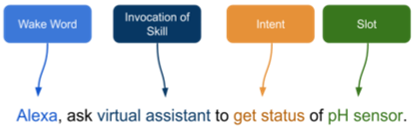
\includegraphics[width=1\linewidth]{fig1.png}
    \caption{Example of Alexa Interaction}
\end{figure}
Currently, there are 12 intents and two slots which are listed in Table 1. There is a “\textit{material}” slot that allows a student to specify a piece of lab equipment and a “\textit{LabTitle}” slot that allows the user to specify which lab to open. 

\begin{table*}[t!]
\caption{Supported Intents of the VLA}
\begin{tabular}{|l|l|l|}
\hline
\textbf{Intent Name} & \textbf{Description} & \textbf{Sample Utterances} \\ \hline
\textbf{Cancel} & Cancels the current task. & Cancel, go back. \\ \hline
\textbf{Help} & Provides users with uses of the skill. Behaves differently depending on the current state of the skill. & Help. \\ \hline
\textbf{Stop} & Closes the skill. & Close, stop. \\ \hline
\textbf{Virtual Assistant} & Gives an introduction to the skill. & What can you do. \\ \hline
\textbf{Get Step} & Announces what step of the lab procedure the user is currently on. & Step, what is my current step, get current step, repeat step, what's the current step, what step am I on. \\ \hline
\textbf{Next Step} & Advances to and reads the next step in the lab procedure. If on the last step, the user is informed, and nothing happens. & What’s next, move on to next step, continue to next step, move on, next step, what’s the next step, continue. \\ \hline
\textbf{Previous Step} & Returns to and reads the previous step in the lab procedure. If on the first step, the user is informed, and nothing happens. & Previous step, last step, go back a step, what was the last step, repeat the previous step. \\ \hline
\textbf{Remaining Steps} & Announces how many remaining steps there are in the lab procedure. & How many more steps, how many remaining steps, number of remaining steps, how many more, how many steps are left. \\ \hline
\textbf{Begin Lab} & Begins a given lab. The title of the lab is given as a slot. & Begin \{LabTitle\}, start \{LabTitle\}, I would like to begin, lab \{LabTitle\}, start lab \{LabTitle\}, begin lab \{LabTitle\}. \\ \hline
\textbf{Exit Lab} & Exits the currently open lab if any. & Quit, quit lab, close lab, exit lab, exit. \\ \hline
\textbf{Materials List} & If a lab is open, list the materials required for that lab. Has a materials slot. & Do I need a \{material\}, list materials, read me the materials list, materials, what materials do I need. \\ \hline
\textbf{Fallback} & The user will be given details on what the skill can do. & If an utterance does not match any of the other intents, this intent is triggered. \\ \hline
\end{tabular}
\end{table*}

We plan on adding support for intents such as calculate, verify answers, check status, and ask TLQ, which will have many slots that will allow for verbal control of the TLQ using the VLA Alexa skill. 
Intents are defined in a JavaScript Object Notation (JSON) structure called the intent schema. The intent schema outlines the intents and slots of the skill as well as examples of what phrases should trigger each intent. The intent schema only defines the basic details of the skill’s intents. The JavaScript (JS) skill code, which implements the functionality of the intents, is not part of the intent schema but exists in an AWS Lambda and is executed on demand.

\subsubsection*{Utterance Profiler Application Programming Interface (API)}

Using the sample utterances defined for the skill’s intents, a natural language processing (NLP) model was trained to learn what similar phrases should trigger an intent. Because the tool infers what intent to trigger based on what the user says, the user is able to engage in a natural dialog with the VLA without the need to memorize specific key phrases. This makes the tool more natural and less intimidating for students to use. To test the interaction model of the VLA skill, Amazon’s Utterance Profiler API was used (“Utterance Profiler API,” n.d.). The Utterance Profiler is given a set of phrases and returns the considered intents to trigger. The sample utterances can then be updated to ensure the correct intent is triggered for a given utterance.
\newpage
\subsubsection*{AWS Lambda}

The AWS Lambda is a serverless computing platform that runs code on demand in response to an event (“AWS Lambda,” n.d.). In the context of the VLA, the triggering event would be the invocation of a skill intent. All skill code is hosted in an AWS lambda. This eliminates the need for any private servers and results in an easily maintained application. 

\subsubsection*{Alexa Gadgets and Raspberry Pi}

Alexa Gadgets are devices that can be controlled via Alexa (smart devices). Using Amazon’s Alexa Gadget Toolkit, anyone can turn any device into an Alexa Gadget (“Understand the Alexa Gadgets,” n.d.). Gadgets can be accessed from an Alexa skill and information can be shared between the gadget and the skill.

Rather than making the TLQ an Alexa Gadget, we choose to use a Raspberry Pi (Raspberry Pi Zero W) to act as an Alexa Gadget (“Alexa-Gadgets-Raspberry-Pi,” n.d.). The Raspberry Pi will then control the TLQ via a micro-USB to USB cable. Since the TLQ is controllable via a keyboard, the Raspberry Pi will be defined as a USB device so that it can act as a keyboard and send keypresses to the TLQ. 

\subsubsection*{Structure of the VLA System}

The user prepares the Echo or smart device to receive an utterance by using the wake word. They can then ask Alexa to perform a task, such as launching the VLA skill. Once the VLA skill is launched, a line of communication is opened between the Alexa Cloud and the Skill code contained in the AWS Lambda.

\begin{figure}[!h]
    \centering
    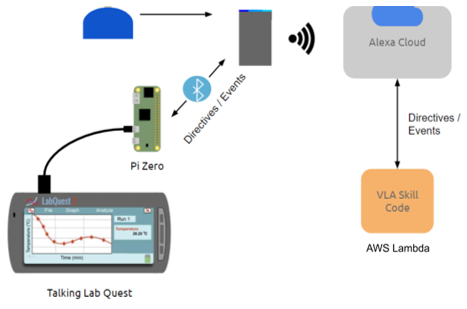
\includegraphics[width=1\linewidth]{fig2.png}
    \caption{Structure of the VLA System and Control of an Accessible Device}
\end{figure}

This allows students to interact with our custom VLA software through the Alexa Smart speaker interface. The user can then give the Echo device a directive which will be relayed through the Alexa cloud to the skill code lambda where it can be processed. Usually, blind students use a USB keyboard to navigate the menus of the TLQ. While many blind students are proficient with keyboards, the interaction could be improved if students were also provided with an option to use their voice. Rather than the students directly using a keyboard to control the TLQ, we are developing a method that allows students to control the TLQ using their voice. This is done using an Alexa smart speaker, custom code in the VLA skill code, and a Raspberry Pi microcontroller that will send simulated keypresses when triggered by the custom VLA skill code. At the same time, the Raspberry Pi will also act as an Alexa Gadget so that it can communicate with the Alexa cloud and smart speaker. The key presses will be simulated using custom scripts and triggered by various VLA skill intents and slots. That is, certain phrases are mapped to certain keyboard presses, allowing the user to navigate the TLQ menus using Alexa. This provides a direct method of controlling the TLQ audibly in a hands-free manner. When the user provides Alexa with an utterance, it is relayed over Wi-Fi to the Alexa Cloud where natural language processing algorithms and the Utterance Profiler determine what was said and which intent/slot should be triggered in the VLA skill code. The skill code then returns directives/\\events to the Alexa Cloud. These directives could be audio responses from the skill or a directive to be passed to the Raspberry Pi. If it is a directive for the Raspberry Pi, it will be passed to the Alexa Echo device over Wi-Fi, then to the Raspberry Pi over Bluetooth. The Raspberry Pi will then simulate certain keypresses to navigate the menus of the TLQ via a micro-USB to USB cable.

\subsubsection*{The adaptability of the VLA System - The VLA Readable Format}

The VLA was designed to improve the lab experience of students with VI and eventually improve the accessibility of science education in general. Thus, the VLA must be flexible enough that users can implement it in their general laboratory work without any AI or software knowledge. To accomplish this goal, we designed the VLA with the ability to read lab files and interpret the contents. Any general lab procedure can be interpreted if written under our well-defined file format, “VLA Readable Format.” The VLA Readable Format is in the style of a markup language and relies on tags to tell the VLA what it should do with a given section of the lab document.

There are two kinds of tags: opening and closing. Opening tags are denoted by surrounding the tag name with the < and > symbols. Closing tags are denoted similarly but with a forward slash immediately following the < symbol. This is similar to other markup languages such as HTML or XML. For example, to define a task in the lab procedure, the appropriate syntax would be <task> … *task contents* ...  </task>. The grouping of an opening tag, the closing tag, and the contents between the tags is called a block. Some blocks support the nesting of other blocks, i.e., subtask blocks can be nested inside of task blocks. Blocks are the foundational bricks from which VLA-readable documents are constructed. All text in a VLA-readable document, with the exclusion of comments, is contained within a block.

\begin{table}[ht]
\caption{Supported Tokens in VLA Readable Format}
\begin{tabular}{|c|l|}
\hline 
\textbf{Token} & \textbf{Description} \\ \hline
< & Opening character of a tag. \\ \hline
> & The closing character of a tag. \\ \hline
/ & Indicates the tag is a closing tag. Immediately follows the ‘<’ token. \\ \hline
: & Denotes the following text is a label. Can only occur inside the opening tag after the tag name. \\ \hline
text & The text contained within a set of opening and closing tags. \\ \hline
name & Name of the tag (materials, procedure, task, etc.). Same as text token but immediately follows ‘<’ or ‘/’ token. \\ \hline
label & The user-defined label of an opening tag. Same as text token but immediately follows ‘:’ token. \\ \hline
\end{tabular}
\end{table}

A VLA-readable document is first passed through a Lexer. The job of the Lexer is to extract the tokens which make up the file and place them in a first-in-first-out (FIFO) list. The order of the tokens in the FIFO list is the same order as they appear in the file. Tokens are the most basic elements of a VLA-readable document. In its current state, the VLA Readable Format has seven tokens.

We plan to add an expression token that will be inside of an equation block. These expressions will be written in either MathML or LaTeX and will have their own tokens, lexicography, grammar, and parsing rules. 

\begin{figure}[h]
    \centering
    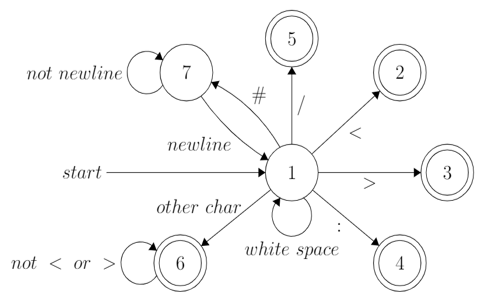
\includegraphics[width=1\linewidth]{fig3.png}
    \caption{Finite-state Machine (FSM) of the VLA Readable Format Design}
\end{figure}

The rules for extracting tokens can be stated using a deterministic finite-state machine (FSM). The goal of a deterministic FSM is to accept or reject a string of symbols by proceeding through a finite sequence of states which is uniquely determined by the string. States and accept states are denoted graphically by a circle and a circle inside a circle, respectively.

If at any time, a symbol is encountered and there is a corresponding path transiting the current state to another state, the path is taken, regardless of whether the state is an accept state or not. If the FSM is in a state and a symbol is encountered with no arrow leaving that state, then if the finite-state machine is in an accept state, it simply accepts. Otherwise, an error would occur, and the string is rejected. A rejected string in the context of the VLA Readable Format would be a syntax error and the VLA would not accept the file as a valid lab document. Note the \# symbol is not a token but can be used in a VLA-readable document to denote a comment. Comments are ignored during parsing and are used to clarify things for any human who is reading or editing a VLA-readable document.

\begin{table}[h!]
\caption{Context-free Grammar for VLA}
\begin{tabular}{|l|}
\hline
\textbf{〈blockList⟩ → 〈block⟩ | 〈block⟩ 〈blockList⟩} \\ \\
\begin{tabular}[c]{@{}l@{}} \textbf{〈block⟩ → 〈tag⟩ 〈tag⟩ | 〈tag⟩} text \textbf{〈tag⟩ | 〈tag⟩ 〈subBlockList⟩} \\ \textbf{〈tag⟩ | 〈tag⟩} text \textbf{〈subBlockList⟩ 〈tag⟩} \end{tabular} \\ \\
\textbf{〈subBlockList⟩ → 〈subBlock⟩ | 〈subBlock⟩ 〈subBlockList⟩} \\ \\
\textbf{〈subBlock⟩ → 〈subblock⟩ | 〈tag⟩ text 〈subBlock⟩ 〈tag⟩} \\ \\
\textbf{〈tag⟩} → < name > | < name: label > | < / name > \\ \hline   
\end{tabular}
\end{table}

After the Lexer places all tokens into a FIFO list, the Parser is responsible for interpreting sequences of tokens. The rules placed on the sequence of tokens are collectively called grammar. The VLA Readable Format has simple grammar. All text in the file must be enclosed in a block, i.e., within an opening and closing tag. Sub-blocks can be nested inside other blocks and include the section, task, and subtask block.

\begin{table*}[th]
\caption{Currently supported block and sub-block types in VLA Readable Format.}
\begin{tabular}{|l|l|l|}
\hline
\textbf{Name} & \textbf{Type} & \textbf{Use} \\ \hline
\textbf{title} & block & The title of the lab. \\ \hline
\textbf{introduction} & block & Introduction to the lab. \\ \hline
\textbf{objectives} & block & List of objectives to be completed by the end of the lab. Each objective is on its own line. \\ \hline
\textbf{materials} & block & List of materials needed for the lab. Each question is on its own line. \\ \hline
\textbf{questions} & block & List of questions. Each question is on its own line. \\ \hline
\textbf{procedure} & block & The lab procedure. \textbf{Section} and \textbf{task} blocks can be nested inside of the \textbf{procedure} block. \\ \hline
\textbf{section} & sub-block & Defines a section of the lab procedure. Must be nested inside of the \textbf{procedure} block. \textbf{Task} blocks can be nested inside of a \textbf{section} block. \\ \hline
\textbf{task} & sub-block & Defines a task to be completed in the lab procedure. Must be nested in a \textbf{section} or \textbf{procedure} block. \textbf{Subtask} blocks can be nested inside of a \textbf{task} block.  \\ \hline
\textbf{subtask} & sub-block & Defines a task to be completed in the lab procedure. Must be nested in a \textbf{task} block. \\ \hline
\end{tabular}
\end{table*}

A VLA-readable document is made up of a list of blocks that themselves may contain sub-blocks. Currently, there are six block types and 3 sub-block types. We plan on expanding this in the future to allow for more customization when writing a lab in the VLA Readable Format. All text tokens from the procedure, section, task, and subtask blocks are placed into a last-in-first-out (LIFO) stack, called the procedure stack, in the reverse order from which they appear in the VLA readable document. Each of these text tokens is considered a step to be completed in the lab procedure. After the VLA readable lab has been parsed, a student will be able to navigate the procedure by using the “next step” and “previous step” intents in the Alexa skill. When the “next step” intent is triggered, the current step (the top of the procedure stack) is popped from the stack, set as the current step, and read aloud by the VLA.  When the “next step” intent is triggered again, the current step is pushed onto a completed stack, and the new top of the procedure task is popped, set as the current step, and read aloud by the VLA. The step marked as the current step is the only step that is ever read allowed by the VLA. When the “previous step” intent is triggered, the current step is pushed back onto the procedure stack and the top of the completed stack is popped, set as the current step, and read aloud by the VLA. The VLA will inform the student if there are no previous or next steps, and neither stack will change.

\begin{figure}[!h]
    \centering
    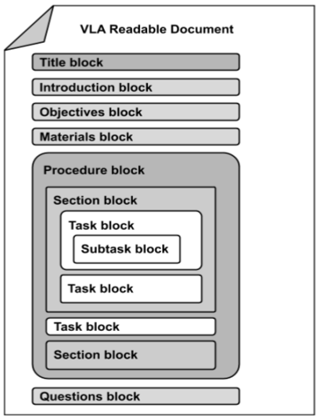
\includegraphics[width=1\linewidth]{fig4.png}
    \caption{Structure of VLA readable document}
\end{figure}

The contents of tags are parsed from the VLA-readable file and handled accordingly. For instance, all task tags will be stored in a list within the AWS Lambda. Students can then navigate the tasks by saying, “next step,” “previous step,” etc. When a student navigates tasks, the VLA will announce the task number and read the related instruction defined within the task tag. 

\begin{figure}[!h]
    \centering
    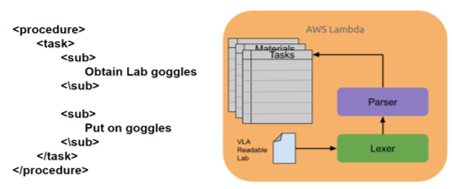
\includegraphics[width=1\linewidth]{fig5.png}
    \caption{An example of a procedure in VLA Readable Format (left) and the resulting document parsing (right)}
\end{figure}

A guideline file, “VLA Readable Format Guide,” has also been developed, providing explicit directions on creating and uploading a file, including the syntax, schemas, and recommended style to keep files consistent for readability and future maintainability. Educators can simply follow the VLA Readable Format Guide to create the lab documents according to the lab contents and import them to the VLA before the lab. The VLA simply gets more knowledgeable about different lab procedures for every document that is imported. No preparation work is needed for students before the lab. With the VLA Readable Format Guide, it requires no technical knowledge to produce and upload VLA-readable files to the VLA system. Having the VLA Readable Format designed and implemented, the adaptability of the VLA system is improved greatly.

\subsection*{VLA System Demonstration}

The VLA system was demonstrated to about 20 blind high-school and college-age students participating in a summer youth training program offered by the Colorado Center for the Blind. Several of these students had taken STEM laboratory courses in the past and had encountered many of the barriers described early on in this paper. These students agreed that, had the VLA had been available for their previous laboratory courses, it would have provided a more independent and hands-on experience. The VLA system was also demonstrated in a presentation at the 2020 Inclusion in Science Learning a New Direction (ISLAND) Conference on disability and STEM, where it received a lot of positive feedback and comments. Additionally, the VLA system was demonstrated in internal meetings at the Sensing, Machine Vision, and Robotics Lab at University of Colorado Denver, and the company Independence Science. 

After the tool was successfully built and tested, the source code of the developed VLA tool was released to GitHub and shared with the public (Watters, J. n.d.). The instruction documents, VLA Readable Format Guide, and a sample laboratory procedure in the VLA Readable Format are shared with the director of the Chemistry lab at the Metropolitan State University of Denver for trial usage. We plan on developing more in-depth testing of the tool where students will actually complete labs with and without the tool and provide feedback. This will help us characterize how this tool enhances the experience of students in the lab and will help us identify issues with the software.

\subsection*{Future Directions}

One of the many difficulties visually impaired students face in the laboratory is recording data in Excel spreadsheets. While there are currently various tools to aid these students with creating and managing spreadsheets, Excel can be a difficult and unnatural tool to use with screen readers as they only tell the user what is in the spreadsheet but offer no direct way to edit it hands-free. We plan on adding several intents to the skill code that would provide Excel or Google Sheets support to the VLA tool. Students would be able to create, edit, and save spreadsheets to their Google Drive account which can be linked to the VLA skill (“Understand Account Linking,” n.d.). This will provide students a completely hands-free method of organizing lab data.

Although the VLA tool was designed with visually impaired students in mind, we feel the tool can be useful for any student in the lab. As such, we would like to add more features to help all students with their lab work. Additional features that benefit all students could be some general knowledge science database, such as a periodic table. Students could ask for the atomic number/weight of certain elements, if an element is a metal, etc.

We also plan on extending the features of the VLA Readable Format to support a simple subset of MathML or LaTeX so that equations can be added into VLA-readable documents. The MathML / LaTeX code would be embedded in a new tag called the equation tag. Additionally, a new “calculate” intent would be added to the VLA Skill code that would allow students to plug values into the equation. The VLA would then compute the solution and speak it back to the user.

Currently, labs must be uploaded directly to the VLA AWS Lambda. This is obviously not ideal as it would be impractical to give all educators access to the skill code. Therefore, we would like to have a system that allows Universities to connect a Google Drive to the tool where all VLA-readable labs would be uploaded. Different classes could then be defined, and labs uploaded to the corresponding folders. We envision students being able to then enable the VLA tool on their Amazon Alexa account and subscribe to courses using a course invitation code or something similar. 

\section*{CONCLUSION}

Our VLA system provides students with a virtual assistant in the lab which can be controlled using natural language rather than memorizing specific keywords or phrases. It can also dictate arbitrary lab procedures at the same pace that students complete their lab work by pausing after each step until the student asks to move on to the next task. It provides students the ability to control laboratory equipment in a completely independent manner via voice command. We are currently developing additional capabilities, including the voice-controlled creation and editing of Excel spreadsheets and the completion of calculations using provided equations. In these ways, our tool greatly increases the accessibility of science labs for the blind and gives students an intuitive method of performing lab work. In conjunction with the TLQ and other accessible tools, our tool improves the lab experience of students with VI, allowing them to take control of their own learning in the lab with minimal aid from sighted lab partners. 

\end{large}
\include{} 
\section*{REFERENCES}\par 

\leftskip 0.25in
\parindent -0.25in 

Alexa-Gadgets-Raspberry-Pi-Samples (n.d.). Retrieved March 07, 2021, from \url{https://github.com/alexa/Alexa-Gadgets-Raspberry-Pi-Samples}

Alexa Skills Kit. (n.d.). Retrieved March 07, 2021, from \url{http://developer.amazon.com/en-US/alexa/alexa-skills-kit}

AWS Lambda. (n.d.). Retrieved March 07, 2021, from \url{https://aws.amazon.com/lambda/}

Field, S., Sarver, M. D., \& Shaw, S. F. (2003). Self-determin\-ation: A key to success in postsecondary education for students with learning disabilities. \textit{Remedial and Special Education,} 24(6), 339-349.

Miner, D. L., Nieman, R., Swanson, A. B., \& Wood, M. (Eds.). (2001). \textit{Teaching chemistry to students with disabilities: A manual for high schools, colleges, and graduate programs.} American Chemical Society, Office of Professional Training.

Rose, D. H., Meyer, A., \& Hitchcock, C. (2005). \textit{The universally designed classroom: Accessible curriculum and digital technologies.} Harvard Education Press.

Supalo, C. A. (2005). Techniques to enhance instructors' teaching effectiveness with chemistry students who are blind or visually impaired. \textit{Journal of Chemical Education,} 82(10), 1513.

Supalo, C. A. (2012). The Next Generation Laboratory Interface for Students with Blindness or Low Vision in the Science Laboratory. \textit{Journal of Science Education for Students with Disabilities,} 16(1), 34-39.

Talking labquest. (n.d.). Retrieved March 07, 2021, from \url{https://www.perkinselearning.org/accessible-science/products/talking-labquest}

Understand Account Linking (n.d.). Retrieved March 07, 2021, from \url{https://developer.amazon.com/en-US/docs/alexa/account-linking/understand-account-linking.html}

Understand the Alexa Gadgets Toolkit. (n.d.). Retrieved March 07, 2021, from \url{https://developer.amazon.com/en-US/docs/alexa/alexa-gadgets-toolkit/understand-alexa-gadgets-toolkit.html}

U.S. Bureau of Labor Statistics (2020) Persons with a disability: labor force characteristics - 2020. (2021, February 24). Retrieved from \url{https://www.bls.gov/news.re-lease/disabl.nr0.htm}

Utterance Profiler API. (n.d.). Retrieved March 07, 2021, from \url{https://developer.amazon.com/en-US/docs/alexa/\\smapi/utterance-profiler-api.html}

Watters, J. (n.d.). MSU-Virtual-Lab-Assistant. Retrieved March 07, 2021, from \url{https://github.com/jacobdwatters/MSU-Virtual-Lab-Assistant}
\end{document}